\documentclass{article} % For LaTeX2e
\usepackage{iclr2024_conference,times}
\pdfminorversion=6
\usepackage[utf8]{inputenc}
\usepackage{amssymb, amsmath, amsthm}
\usepackage{thmtools, mathtools, mathrsfs}
\usepackage{amsfonts}       % blackboard math symbols
\usepackage{forloop}
\usepackage{stmaryrd}
\usepackage{natbib}
\setcitestyle{square, comma, numbers,sort&compress, super}
\usepackage{subcaption}
\usepackage{graphicx}
\usepackage{caption}
\usepackage{float}
\usepackage{bm}
\usepackage{tikz}
\usepackage{tikz-cd}
\usepackage[T1]{fontenc}    % use 8-bit T1 fonts
\usepackage{hyperref}       % hyperlinks
\usepackage{url}            % simple URL typesetting
\usepackage{booktabs}       % professional-quality tables
\usepackage{nicefrac}       % compact symbols for 1/2, etc.
\usepackage{microtype}      % microtypography
\DeclareGraphicsExtensions{.pdf,.png,.jpg,.mps,.eps,.ps}
\graphicspath{{../figures/}}

\newcommand{\defvec}[1]{\expandafter\newcommand\csname v#1\endcsname{{\mathbf{#1}}}}
\newcounter{ct}
\forLoop{1}{26}{ct}{
    \edef\letter{\alph{ct}}
    \expandafter\defvec\letter
}

% captial \vA
\forLoop{1}{26}{ct}{
    \edef\letter{\Alph{ct}}
    \expandafter\defvec\letter
}

\newcommand{\dm}[1]{\ensuremath{\mathrm{d}{#1}}} % dx dy dz dmu
\newcommand{\RN}[2]{\frac{\dm{#1}}{\dm{#2}}} % (Radon-Nikodym) derivative
\newcommand{\PD}[2]{\frac{\partial #1}{\partial #2}} % partial derivative
\newcommand{\overbar}[1]{\mkern 1.5mu\overline{\mkern-1.5mu#1\mkern-1.5mu}\mkern 1.5mu}
\newcommand{\win}{\vW_{\text{in}}}
\newcommand{\wout}{\vW_{\text{out}}}
\newcommand{\bout}{\vb_{\text{out}}}
\newcommand{\reals}{\mathbb{R}}

\newcommand{\manifold}{\mathcal{M}}

\DeclareMathOperator{\relu}{ReLU}

\newcommand{\probP}{\text{I\kern-0.15em P}}

\newtheorem{theorem}{Theorem}
\newtheorem{prop}{Proposition}
\theoremstyle{definition}
\newtheorem{definition}{Definition}
\theoremstyle{remark}
\newtheorem{remark}{Remark}

\title{RNNs with gracefully degrading continuous attractors}

% Authors must not appear in the submitted version. They should be hidden
% as long as the \iclrfinalcopy macro remains commented out below.
% Non-anonymous submissions will be rejected without review.


\newcommand{\fix}{\marginpar{FIX}}
\newcommand{\new}{\marginpar{NEW}}

%\iclrfinalcopy % Uncomment for camera-ready version, but NOT for submission.
\author{%
    \'Abel ~S\'agodi, Piotr Sok\'o\l, Il Memming Park \\
    %\thanks{Use footnote for providing further information about author (webpage, alternative address).} \\
    \\
    Champalimaud Centre for the Unknown\\
    Champalimaud Foundation, Lisbon, Portugal\\
    \texttt{\{abel.sagodi,piotr.sokol,memming.park\}@research.fchampalimaud.org} \\
}

\begin{document}

%keywords: 
%neural computation, robustness, bifurcation analysis, exploding gradient problem, continuous attractors, persistence of invariant manifolds 
    
%TLDR


\maketitle

\begin{abstract}
Attractor networks are essential theoretical components in recurrent networks for memory, learning, and computation.
However, the continuous attractors that are essential for continuous-valued memory suffer from structural instability---infinitesimal changes in parameter can destroy the continuous attractor.
Moreover, the perturbed system can exhibit divergent behavior with associated exploding gradients.
This poses a question about the utility of continuous attractors for systems that learn using gradient signals.
%This poses a problem in biological neural networks, as they are constantly subjected to perturbations caused by noise. Certain systems (e.g. systems with an unbounded attractor) can be perturbed in such a way, that not only do they bifurcate, but start exhibitung divergent behavior, which is especially problematic for systems that are learning (for example under gradient descent).
To address this issue, we use Fenichel's persistence theorem from dynamical systems theory to show that bounded attractors are stable in the sense that all perturbations maintain the stability.
This ensures that if there is a restorative learning signal, there will be no exploding gradients for any length of time for backpropagation.
In contrast, unbounded attractors may devolve into divergent systems under certain perturbations, leading to exploding gradients.
This insight also suggests that there can exist homeostatic mechanisms for certain implementations of continuous attractors that maintain the structure of the attractor sufficiently for the neural computation it is used in.
Finally, we verify in a simple continuous attractor that all perturbations preserve the invariant manifold and demonstrate the principle numerically in ring attractor systems.
\end{abstract}


%\section{Submission of papers to NeurIPS 2023}
%
%Please read the instructions below carefully and follow them faithfully. \textbf{Important:} This year the checklist will be submitted separately from the main paper in OpenReview, please review it well ahead of the submission deadline: \url{https://neurips.cc/public/guides/PaperChecklist}.


\section{Introduction}
%NeurIPS requires electronic submissions.  The electronic submission site is
%\begin{center}
%  \url{https://cmt3.research.microsoft.com/NeurIPS2020/}
%\end{center}

Recurrent neural/neuronal networks (RNNs) can process sequential observations and model temporal dependencies of arbitrary length.
At the same time, they are fundamentally limited by their finite-sized hidden states which form the only channel between the past and the future.
To store information over a long period of time, as many difficult tasks demand, RNNs can learn or be designed to have ``persistent memory''.
When the information of interest is continuous-valued, a natural solution is to use continuous attractors.
Continuous attractors are prevalent in theoretical neuroscience as tools to model neural representation and computation ranging from internal representations of head directions and eye positions to perceptual decision-making and working memory~\cite{Khona2022}.
Continuous attractors are also at the core of long short-term memory (LSTM)~\cite{Greff2017} units and the neural Turning machine (NTM)~\cite{Graves2014} to provide digital computer memory like properties not natural to recurrent networks. % with many applications such as meta-learning~\cite{Santoro2016}.
In fact, the critical weakness of continuous attractors is their inherent brittleness as they are rare in the parameter space, i.e., infinitesimal changes in parameters destroys the continuous attractor structures implemented in RNNs~\cite{seung1996,Renart2003}, even if with biologically plausible asymmetric connections are used to construct them \citep{darshan2022}.
However, not all RNN implementations of continuous attractors behave similarly in their brittleness.

We found that in the space of RNNs, some have neighbourhoods with highly undesirable exploding gradients. We will describe some continuous attractors which have such neighbourhoods.
Consider an RNN (without input or output for now) expressed in continuous time as an ordinary differential equation:
\begin{align}\label{eq:TLN}
    \dot{\vx} = -\vx + \left[ \vW \vx + \vb \right]_{+}
\end{align}
where $\vx \in \reals^d$ is the hidden state of the network, $\vb > 0$ is the bias, and $[\cdot]_{+} = \max(0,\cdot)$ is the threshold nonlinearity per unit.
In discrete time, this corresponds to a ReLU RNN (see Sec.~\ref{sec:rnn:integration}).
The non-trivial activity of this network is limited to the (non-negative) first quadrant, outside of which the hidden state decays to the origin.

When $d=2$, we can build two kinds of continuous attractors.
First, through positive feedback, $\vW = [0, 1; 1, 0]$ and no bias $\vb = \mathbf{0}$, we can create a continuous attractor, i.e., $\dot{\vx} = 0$ on the $x_1 = x_2 \geq 0$ half-line, and surrounding attractive flow (Fig.~\ref{fig:ublabla}A left).
We refer to it as an \textbf{unbounded line attractor (UBLA)}.
For any point on the line attractor, linearization results in eigenvalues $0$ and $-2$, corresponding to the zero flow and attractive flow respectively.
When $\vW$ is perturbed, the null eigenvalue can easily become non-zero and the continuous line attractor disappears.
If it becomes negative, the system bifurcates to a stable fixed point at the origin (Fig.~\ref{fig:ublabla}A bottom).
However, if it becomes positive (Fig.~\ref{fig:ublabla}A top), \emph{the resulting flow diverges to infinity along the diagonal}.
Corresponding to the divergent flow, the backpropagating gradient over time exponentially grows in magnitude, thus rendering gradient descent impractical without truncation in time.

The second kind of continuous attractor is created through negative feedback.
By choosing $\vW = [0, -1; -1, 0]$ and $\vb = [1; 1]$, we get $\dot{\vx} = 0$ on the $x_1 = -x_2 + 1$ line segment in the first quadrant as the continuous attractor.
We refer to it as the \textbf{bounded line attractor (BLA)}.
Again, linearization on the attractor shows two eigenvalues, $0$ and $-2$, and perturbations again cause the null eigenvalue to be non-zero and the line attractor disappears.
However, surprisingly, the bifurcations are  qualitatively different.
It either bifurcates into a single stable fixed point (Fig.~\ref{fig:ublabla}B top) or two stable fixed points separated with a saddle node in between (Fig.~\ref{fig:ublabla}B bottom).
Neither of these two cases show a divergent flow, but rather consists of one or two basins of attraction.
It implies only vanishing gradients for this system and \textbf{exploding gradients will not be present for an arbitrarily long time}.

\begin{figure}[tbhp]
  \centering
  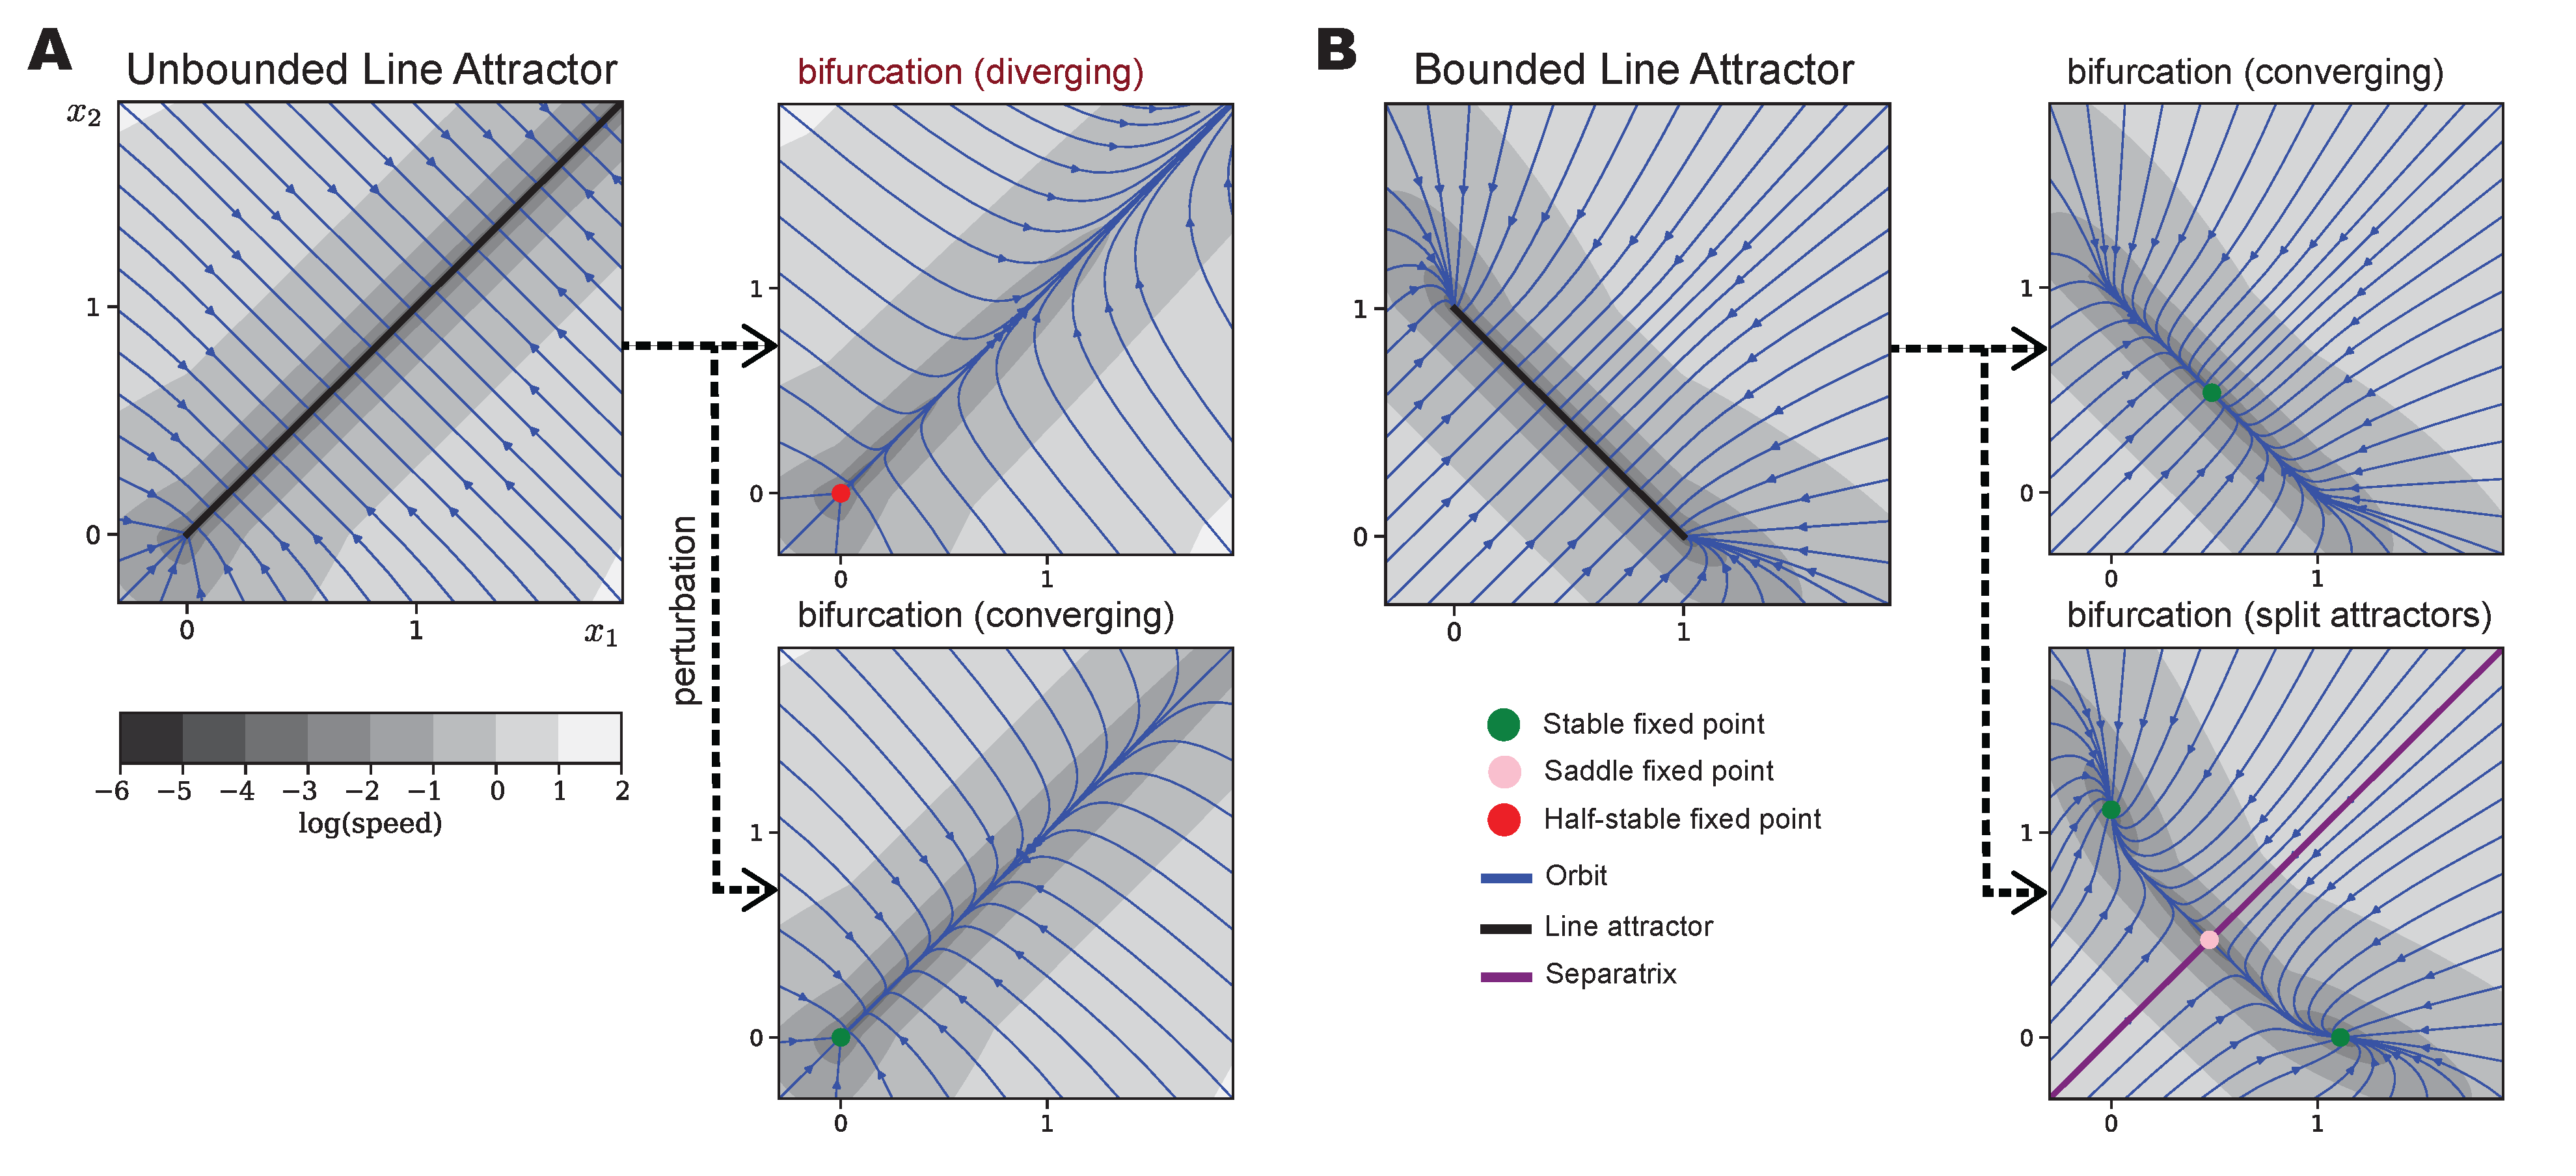
\includegraphics[width=\textwidth]{UBLABLA}
  \caption{Motivating case study of the two systems implementing the same computation but one near exploding gradients.
    Phase portraits for unbounded and bounded linear attractors~\eqref{eq:TLN}.
    Under perturbation of parameters, each of them can bifurcate to one of the two potential systems without the continuous line attractor.
    Note that the parameters for the UBLA are near a diverging system associated with exploding gradient behavior.
% Behavior and bifurcations of the unbounded and bounded line attractors.  Some example orbits are shown with blue lines for each system while the log of the speed in state space is indicated with a grayscale gradient.
%   (Left) Example orbits  for a ReLU RNN implementation of an unbounded line attractor (black line, see Sec. ~\ref{sec:ubla}). This system can bifurcate in two types of dynamics. (Upper arrow) The first type of perturbation leads to a divergent systems with orbits going to positive infinity for all starting positions (except a single orbits that end up at the origin).
%    (Lower arrow) The second type of perturbation leads covergent dynamics with all orbits converging at the origin.
%  (Right from red line) Example orbits (blue lines) for a ReLU RNN implementation of an bounded line attractor (black line, see Sec ~\ref{sec:bla}). This system can bifurcate into two systems with non-zero probability.
%  (Upper arrow) The first type of perturbation leads to a system with a single fixed point (pink).
%  (Lower arrow) The second type of perturbation leads to a system with three fixed points.
}
  \label{fig:ublabla}
\end{figure}

Avoiding exploding gradients is of paramount importance in the context of long-range temporal learning (Sec.~\ref{sec:imp:ML}).
Learning generally induces stochasticity in parameters, while spontaneous synaptic fluctuations are present in biological neuronal networks (Sec.~\ref{sec:imp:neuroscience}).
Given these observations, we predict that BLA would be a more stable motif for computation than UBLA in the presence of noise and continuous learning.
Since BLA, but not UBLAs, avoids exploding gradients, if the desired computation requires a line attractor of finite range, BLA would be both easier to maintain and learn.
Is this only true for ReLU parameterized RNNs, or does it generalize?

In this paper, we lay out a new theory of general continuous-valued memory in the context of learning to answer the following questions:
\begin{enumerate}
    \item Can we avoid exploding gradients under parameter perturbation?
    \item Do we need to worry about the brittleness of the continuous attractor solutions in practice?
\end{enumerate}
Our theory provides answers to both questions under mild assumptions in an architecture agnostic manner.
Using Fenichel's invariant manifold theorem, we derive a sufficient condition for RNNs implementing continuous attractors to remain free of exploding gradients.
Moreover, even after a bifurcation, these RNNs still approximately behave like the original continuous attractor for a while.
Together these theoretical results practically nullify the concern of the fine tuning problem in theoretical neuroscience and suggest general principles for evaluating and designing new architectures and initialization strategies for RNNs in machine learning.

%\section{Background}
%\subsection{Dynamical systems and gradient propagation}
%\subsection{Structural stability and bifurcations}

\section{Theory of gracefully degrading continuous attractors}\label{sec:theory}
In this section, we apply Fenichel's work on invariant manifolds to RNNs and translate the results for the machine learning and theoretical neuroscience audience.

\subsection{Invariant Continuous Attractor Manifold Theory}\label{sec:imt}
We start by formulating RNNs implementing a continuous attractor in continuous time: $\dot{\vx} = \vf(\vx)$.
Let $l$ be the intrinsic dimension of the manifold of equilibria that defines the continuous attractor.
We will reparameterize the dynamics around the manifold with coordinates $\vy \in \reals^l$ and the remaining ambient space with $\vz \in \reals^{d-l}$.
To describe an arbitrary bifurcation of interest, we introduce a sufficiently smooth function $g$ and a bifurcation parameter $\epsilon \geq 0$, such that the following system is equivalent to the original ODE:
\begin{align}\label{eq:fenichel:flow}
    \dot{\vy} &=           \epsilon  \vg(\vy, \vz, \epsilon) \qquad \text{(tangent)}\\
    \dot{\vz} &= \hphantom{\epsilon} \vh(\vy, \vz, \epsilon) \qquad \text{(normal)}
\end{align}
where $\epsilon = 0$ gives the condition for the continuous attractor $\dot{\vy} = \mathbf{0}$.
We denote the corresponding manifold of $l$ dimensions $\manifold_0 = \{(\vy,\vz) \mid \vh(\vy,\vz,0) = 0\}$.

We need the flow normal to the manifold to be hyperbolic, that is \emph{normally hyperbolic}, meaning that the Jacobians $\nabla_\vz \vh$ evaluated on any point on the $\manifold_0$ has $d-l$ eigenvalues with non-zero real parts, and $\nabla_\vy \vg$ has $l$ eigenvalues with zero real parts.
More specifically, for continuous attractors, the real part of the eigenvalues of $\nabla_\vz \vh$ will be negative, representing sufficiently strong attractive flow toward the manifold.
Equivalently, for the ODE, $\dot{\vx} = \vf(\vx)$, the variational system is of constant rank, and has exactly $l$ eigenvalues with negative real parts and $(n-l)$ eigenvalues with zero real parts everywhere along the continuous attractor.

\begin{figure}[bthp]
  \centering
  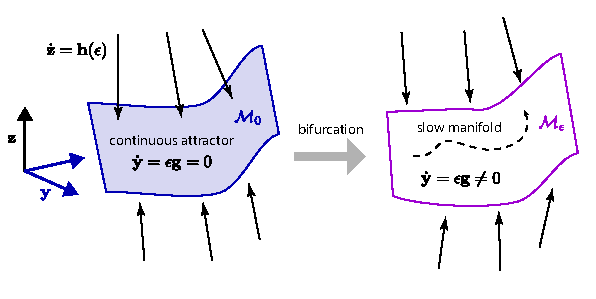
\includegraphics{FenichelThm.pdf}
  \caption{
    Fenichel's invariant manifold theorem applied to compact continuous attractor guarantees the flow on the slow manifold is locally invariant and continues to be attractive.
    The dashed line is a trajectory ``trapped'' in the slow manifold (locally invariant).
  }
  \label{fig:fenichel}
\end{figure}

When $\epsilon > 0$, the continuous attractor bifurcates away.
What can we say about the fate of the perturbed system?
The continuous dependence theorem~\cite{Chicone2006} says that the trajectories will change continuously as a function of $\epsilon$ without a guarantee on how quickly they change.
Moreover, the topological structure and the asymptotic behavior of trajectories change discontinuously due to the bifurcation.
Surprisingly there is a strong connection in the geometry due to Fenichel's theorem~\cite{fenichel1971}.
We informally present a special case due to~\cite{Jones1995}:
\begin{theorem}[Fenichel's Invariant Manifold Theorem]
Let $\manifold_0$ be a connected, compact, normally hyperbolic manifold of equilibria originating from a sufficiently smooth ODE.
For a sufficiently small perturbation $\epsilon > 0$, there exists a manifold $\manifold_\epsilon$ diffeomorphic to $\manifold_0$ and locally invariant under the flow of \eqref{eq:fenichel:flow}.
Moreover, $\manifold_\epsilon$ has corresponding smoothness.
\end{theorem}

The manifold $\manifold_\epsilon$ is called the \emph{slow manifold} which is no longer necessarily a continuum of equilibria.
However, the local invariance implies that trajectories remain within the manifold except potentially at the boundary.
Furthermore, the non-zero flow on the slow manifold is slow and given in the $\epsilon \to 0$ limit as $\RN{\vy}{\tau} = \vg(c^\epsilon(\vy), \vy, 0)$ where $\tau = \epsilon t$ is a rescaled time and $c^\epsilon(\cdot)$ parameterizes the $l$ dimensional slow manifold.
In addition, the stable manifold(s) of $\manifold_0$ are similarly approximately maintained~\cite{Jones1995}, allowing the continuous attractor to remain attractive.

These conditions are met (up to numerical precision) for the BLA example in Fig.~\ref{fig:ublabla}B.
As the theory predicts, BLA bifurcates into a 1-dimensional slow manifold (dark colored regions) that contains fixed points, and overall still attractive.
On the contrary, the UBLA does not satisfy the compactness condition, hence the theory does not predict its persistence.
Importantly, the ``slow'' flow on the perturbed system is not bounded.

In practice, the sufficient conditions for RNNs implementing continuous attractors to have this graceful breakdown is for the continuous attractor manifold to be of finite dimension throughout, connected, and bounded. 
However, in systems with an invariant manifold with dimension at least three, it is possible that a slow manifold with chaotic dynamics is created through a perturbation. This would have as consequence that the perturbed system acquires positive Lyapunov exponents (corresponding to the chaotic orbit), which then can still lead to exploding gradients.

\subsection{Implications on Machine Learning}\label{sec:imp:ML}
Extending the memory time constant of RNNs have long been an important area of research with much focus on random weights~\cite{Legenstein2007,Goldman2009,Toyoizumi2011,Kerg2019,Chen2018,Henaff2016,Rusch2021,arjovsky2016}.
Various initializations for the recurrent weights have been proposed to help learning: initialization with the identity matrix \citep{le2015}, with a random orthogonal matrix \citep{saxe2014,Henaff2016}, with a unitary matrix \citep{arjovsky2016} and with a block diagonal weight matrix that creates a quasi-periodic system with limit cycles \citep{Sokol2019a}.
However, despite the capacity to maintain representation of continuous quantities for arbitrary duration of time, continuous attractor mechanism has not been pursued in machine learning research because of its brittleness.
The stochasticity in gradients inherited from the training data, regularization strategy, and multi-task learning objectives act as a perturbation on the recurrent dynamics, and continuous attractors break down even if it could be learned.
Remedies emerged in machine learning to hard-code continuous-valued memory structures within the RNNs---e.g., the cell state in vanilla LSTM.
However, our theory shows that the geometric structure of the manifold and the flow around the manifold play a critical role in enabling gradient descent learning of continuous attractors using standard methods such as backpropagation through time (BPTT)~\cite{Toomarian1991}.

It is well known that asymptotic exploding gradients comes from positive Lyapunov exponents~\cite{Mikhaeil2022,Vogt2022,Engelken2023}.
It has also been pointed out that bifurcations can cause arbitrarily large gradients~\cite{doya1993} as well as discontinuity in the Lyapunov spectrum~\cite{Park2023a}.
These gradient propagation theories suggested that bifurcations should be avoided, including the continuous attractors.

As far as we know, there is no architecture agnostic theory describing the loss landscape around RNN solutions.
We remark that due to the singular nature of the center manifold that supports the continuous attractor, the usual analysis approach of linearization fails.
\emph{Our theory successfully connects the invariant manifold theory and the gradient signal propagation theory in RNNs to describe two types of loss landscape around continuous attractor solutions.}
In one case, when the theorem holds, the landscape is shallow in all directions due to (asymptotically) vanishing gradients induced by the attractor structure---we have the gracefully degrading continuous attractor.
On the other case, we can find examples where the theorem does not hold, and the continuous attractor solution is at the boundary of network configurations with exploding gradients, meaning the loss landscape is very steep in some directions.

While exploding gradients would prevent gradient descent to correct for deviations from the optima,
for gracefully degrading ones, one can apply restorative forces via gradient descent to be in the vicinity of the brittle continuous attractor solution (see Sec.~\ref{sec:exp:maintaining}).


\subsection{Implications on Neuroscience}\label{sec:imp:neuroscience}
Continuous attractors are biologically plausible, theoretically elegant, consistent with neural recordings, and avoids the asymptotic exploding and vanishing gradient problem~\cite{Park2023a}.
As a conceptual tool in computational and theoretical neuroscience, continuous attractors are widely used when working memory of continuous values is needed~\cite{Dayan2001,Burak2009,Khona2022}.
When used to accumulate stimulus, continuous attractors are also called neural integrators that are hypothesized to be the underlying computation for the maintenance of eye positions, heading direction, self-location, target location, sensory evidence, working memory, decision variables, to name a few~\cite{seung1996,Seung2000,Romo1999}.
Neural representation of continuous values have been observed as persistent activity in the prefrontal cortex of primates, ellipsoid body of the fly, and hypothalamus~\cite{Romo1999,Noorman2022,Nair2023}.
A typical computational implementation of a continuous attractor are bump attractor network models which require a mean-field limit~\cite{Skaggs1995,Camperi1998,Renart2003} and finite sized networks with threshold linear units \cite{Noorman2022,Spalla2021}, see also Sec.~\ref{sec:hd}.

However, the so-called ``fine-tuning problem'' describing the theoretical and practical brittleness of continuous attractors was recognized in~\citep{seung1998}.
Since biological neural systems have constantly fluctuating synaptic weights~\cite{shimizu2021}, this has been a big puzzle in the field.
There have been efforts and remedies to lessen the degradation for particular implementations, often focusing on keeping the short-term behavior close to the continuous attractor case~\cite{Lim2012,Lim2013,Boerlin2013,Koulakov2002,Renart2003}.

Our theory shows that not all continuous attractors are born equal, and there are gracefully degrading continuous attractors.
In finite time, trajectories are well-behaved, contrary to the asymptotic behavior captured by the Lyapunov exponents.
Animal behavior is finite time in nature and the longer the temporal distance the harder it is to learn in general.
The conditions are favorable in the recurrent neuronal networks: (1) mutual inhibition is widely present and evidence points to inhibition dominated dynamics,
(2) the neural state space is bounded due to physiological constraints-- by a non-negative firing rate below and a maximum firing rate above.

%Given an $d$-dimensional continuous attractor manifold embedded within a recurrent dynamics of $n$-dimensions, it supports persistent continuous memory of $d$-dimension.
%There are $d$ zero Lyapunov exponents corresponding to the perturbations tangent to the manifold, coinciding with the memory representation, and $(n-d)$ negative Lyapunov exponents that expresses the attractive nature.
%In theory, the topology of the manifold can be arbitrary, ideally matching the desired structure of the target variables.

\section{Experiments}
\subsection{Continuous-valued click integration task}\label{sec:task:continuous-clicks}
Although there are several standard benchmark tasks for temporal dependence learning with memory components,
due to the discrete nature of the relevant stimulus space, the solutions do not necessarily require a continuously-valued memory.
We designed a simple integration task where one of the optimal solutions is the continuous attractor.

We extend the Poisson clicks task which has been used for studying perceptual decision making~\cite{brunton2013}.
Neural integrators are considered to be crucial for the task for accumulating evidence over time and maintaining a continuous representation of the accumulated evidence.
For our experiments, we used discrete time representations over $T$ time bins and the real-valued\footnote{Approximated as single precision IEEE 754 floating point.} stimulus encoded as difference of two non-negative values:
\begin{align}
    I_{t,i} &= m_{t,i} \cdot u_{t,i} 
            & \qquad \text{(continuous clicks)}
    \\
    O^\ast_{t} &= \sum_{s=0}^{t} \left(
        I_{s,1} - I_{s,2}
        \right)
            & \qquad \text{(desired output)}
\end{align}
where $m_{t,i}$ are independent Bernoulli random variables with probability $0.2$ and $u_{t,i}$ are independent random variables with uniform distribution on the unit interval.
We used mean squared error (MSE) of the 1-dimensional output over time as the loss function over all time bins.
We used $T=500$ time bins per trial unless specified otherwise.
The gradients were computed in batch mode with $1000$ randomly generated trials.
The main challenges of this task are (1) addition and subtraction and (2) maintain the accumulated clicks for extended period of time.

%The inputs for the clicks task are incoming clicks in two channels ($K=2$) and are given as follows.
%The non-zero inputs follow a Poisson distribution with given rates.
%At such time points, an input is sampled from $[0,1]$.
%The task is to output the difference between the two inputs in the two channels. 

%A noisy version of the task also includes noise added to a part of the input, without alternation to the target output, i.e., the noise added to the system should be ignored by the system.

\subsection{RNN solutions to the integration task}\label{sec:rnn:integration}
We use vanilla RNN implementations with the standard parameterization:
%An RNN \citep{elmanFindingStructureTime1990} consists of a $N \times N$ transition matrix $W$, an $L \times N$ decoder matrix $\wout$ (where $L$ is the output dimension), a $N \times K$ encoder matrix $\win$ (where $K$ is the input dimension), and a bias $b$ for the hidden state and $\bout$ for the output.
% If either the output or input is categorical, $M$ (respectively $N$) is the number of classes, and we use a one-hot representation. 
%As the RNN ingests a sequence, at each timestep it updates to a hidden state $h$, and using the hidden state and the decoder matrix, produces outputs $y$:
\begin{equation}
  \begin{aligned}
	\vx_t &= \sigma(\win \vI_t + \vW \vx_{t-1} + \vb) \label{eq:RNN:discrete}\\
	O_t &= \wout \vx_t + \bout
  \end{aligned}
\end{equation}
where $\vx_t \in \reals^d$ is the hidden state, $\vI_t \in \reals^K$ is the input,
$\sigma: \reals \to \reals$ an activation function which acts on each of the hidden dimension, and
$\vW, \vb, \win, \wout, \bout$ are parameters.
Assuming an Euler integration with unit time step, the discrete-time RNN of \eqref{eq:RNN:discrete} corresponds to the ODE:
\begin{align}
    \dot{\vx} &= -\vx + \sigma(\win \vI + \vW \vx + \vb) \label{eq:RNN:continuous}
\end{align}

For tractable analysis, we consider $2$ dimensional systems with ReLU activation.
We study three different RNN implementations of an integrator, the Identity RNN (iRNN), UBLA and BLA.
On the original clicks task the UBLA and BLA networks count the click differences directly, while iRNN counts the clicks separately and then subtracts these representations through the output mapping.
The behaviors of UBLA and BLA in the absence of stimulus are shown in Fig.~\ref{fig:ublabla}, while the behavior of the iRNN is trivial since there is no flow. These networks are defined as follows.

\paragraph{Identity RNN}
\label{sec:ubpa,sec:iRNN}
%This is an RNN with the identity matrix as its recurrent weights  with two hidden units. 
\begin{equation}\label{eq:irnn}
\win = 
\begin{pmatrix}
1  &  0 \\
0 &  1
\end{pmatrix}, \
\vW = 
\begin{pmatrix}
1  &  0 \\
0  &  1
\end{pmatrix}, \
\wout = 
\begin{pmatrix}
-1  \\  1 
\end{pmatrix}, \
\vb = 
\begin{pmatrix}
0  \\ 0
\end{pmatrix}, \
\bout = 0.
\end{equation}

%The system has the whole state space as its invariant manifold.

\paragraph{Unbounded line attractor}
\label{sec:ubla}
\begin{equation}\label{eq:ubla}
\win = \alpha
\begin{pmatrix}
-1  &  1 \\
-1  &  1
\end{pmatrix}, \
\vW = 
\begin{pmatrix}
0  &  1 \\
1  &  0
\end{pmatrix}, \
\wout = \frac{1}{2\alpha}
\begin{pmatrix}
1  \\  1 
\end{pmatrix}, \
\vb = 
\begin{pmatrix}
0  \\  0
\end{pmatrix}, \
\bout = -\frac{\beta}{\alpha}.
\end{equation}

While the line attractor is unbounded from above, it only extends to the center from below.  The  step size along line attractor $\alpha$ determines the maximum number of clicks as the difference between the two channels; the capacity is $\beta/\alpha$ number of clicks.

\paragraph{Bounded line attractor}\label{sec:bla}
We formulate this implementation of a bounded integrator with a parameter that determines step size along line attractor $\alpha$. Analogously as for UBLA, these parameters determine the capacity of the network.
The inputs push the input along the line attractor in two opposite directions, see below. UBLA and BLA need to be initialized at $\beta(1,1)$ and $\tfrac{\beta}{2}(1,1)$, respectively, for correct decoding, i.e., output projection.

\begin{equation}\label{eq:bla}
\win = \alpha
\begin{pmatrix}
-1  &  1 \\
1  &  -1
\end{pmatrix}, \
\vW = 
\begin{pmatrix}
0  &  -1 \\
-1  &  0
\end{pmatrix}, \
\wout = \frac{1}{2\alpha}
\begin{pmatrix}
1  \\  -1 
\end{pmatrix}, \
\vb = \beta
\begin{pmatrix}
1 \\  1 
\end{pmatrix}, \
\bout = 0.
\end{equation}

\subsection{Asymmetric loss landscape due to exploding gradients}
To illustrate the effect of bifurcations from continuous attractor solution, we take a 1-dimensional slice of the loss surface.
Specifically, we take the self-recurrent connection and systematically vary:
\begin{align}
    \vW_{1,1} \leftarrow \vW_{1,1} + \Delta.
\end{align}
The result is shown in Fig.~\ref{fig:maintenance}A.
For UBLA and iRNN, positive perturbations shows exponentially increasing loss due to the bifurcation to an exploding gradient dynamical system.
In all other cases, including all perturbations of BLA, leads to vanishing gradient, hence the loss is bounded.

\begin{figure}[thbp]
  \centering
  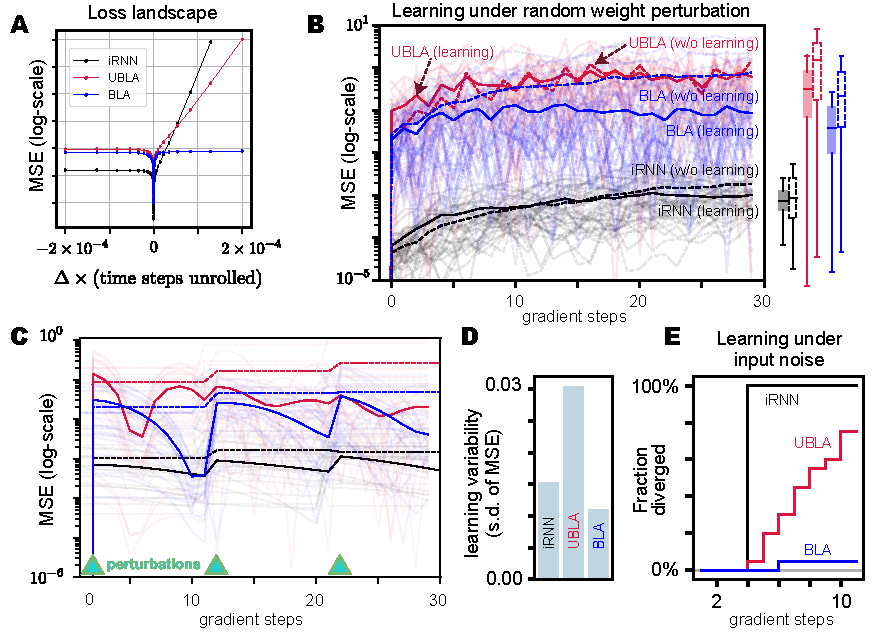
\includegraphics[width=\textwidth]{threeIntegrators.pdf}
  \caption{
  Comparing three continuous attractor solutions to the click integration task.
  (A) Single parameter perturbation showing exploding gradients for iRNN and UBLA.
  (B) Effect of gradient descent in repairing the continuous attractor. RNNs without gradient descent (dashed line) are shown for reference. Box plots show distribution of the loss for the last 10 steps.
  (C) Interleaved weight perturbations showing gradual recovery for BLA and iRNN.
  (D) High variability across time of UBLA and iRNN due to exploding gradients.
  (E) Noise injected to objective induces gradient descent to drive solutions to diverge away.
  }
  \label{fig:maintenance}
\end{figure}


\subsection{Bifurcation probability and random perturbations}
We consider all parametrized perturbations of the form $ \vW \leftarrow \vW + \vV$ for a random matrix $\vV\in \mathbb{R}^{2\times 2}$.
The BLA can bifurcate in the following systems, characterized by their invariant sets: a system with single stable fixed point, a system with three fixed points (one unstable and two stable) and  a system with two fixed points (one stable and the other a half-stable node) and a system with a (rotated) line attractor. 
Only the first two bifurcations (Fig. ~\ref{fig:ublabla}) can happen with nonzero chance for arbitrary the type of perturbations we consider.
The  perturbations that  leave the line attractor intact and or two a system with two fixed points have measure zero in parameter space.
The types of perturbation with measure zero are codimension 2 bifurcations.
The perturbation that results in one fixed point happen with probability $\frac{3}{4}$, while perturbations lead to a system with three fixed points with probability $\frac{1}{4}$.




\subsection{Maintaining a neural integrator}\label{sec:exp:maintaining}
To investigate the differential effect of gradient descent on the three neural integrator models, we performed three learning experiments using the continuous-valued click integration task.

In the first experiment, Gaussian random noise is injected to all parameters inducing a constant diffusion of the parameters.
This emulates the biological synaptic variability.
Fig.~\ref{fig:maintenance}B shows that for BLA, gradient descent (with constant learning rate, chosen from a grid search) was able to counter the diffusion.
Note that the magnitude of perturbation were identical for all networks, but iRNN is more robust in terms of MSE.
The distribution of MSE for the task can be used as proxy for the misadjustment from the optimal solution.
BLA with learning has superior misadjustment to UBLA and BLA without learning.

To dissociate the effect of misadjustment from gradient descent and external perturbation, we interleaved a larger perturbation with 10 gradient steps.
Fig.~\ref{fig:maintenance}C shows consistent learning in the average MSE for BLA and iRNN, but not in UBLA.
The individual runs indicate larger variability induced by learning over time, which we quantify in Fig.~\ref{fig:maintenance}D.
iRNN and UBLA both have larger learning noise than BLA, consistent with the absence of exploding gradient configuration around the optimum.

Finally, we investigated the effect of learning when perturbations are induced by the backpropagated gradient which is structured by the recurrent dynamics.
To inject noisy gradients naturally, we added noise to the input to the first 10 time steps during the trial that were not integrated.
Then we looked for networks that diverged due to exploding gradients which we identify as having a loss of 1 or higher. %normally loss is very low, zero for the perfect integrators
Fig.~\ref{fig:maintenance}E shows that UBLA and iRNN quickly diverges under gradient descent than the BLA.
%$This is because the noise sometimes pushes the UBLA to the regime with divergent dynamics which leads to exploding gradients, which then causes the weights to make bigger jumps.


%noisy learning experiments
%We investigate the effects of noise to the inputs on the loss and the effect of such noise on the learning/adjustment of the parameters during gradient descent starting from the perfect solutions to the task.
%We inject a pulse of 10 steps of inputs sampled from the uniform distribution and take a gradient step in the direction of the accumulated gradient.

The parameters that were used for the effects of input- and parameter-type noise are summarized in Table \ref{tab:params}.
The bias parameters of the UBLA and BLA networks were set to $\beta=100$, while $\alpha=1$. 
The hidden state at the beginning of a trial is a learnable parameter. 
The optimal learning rates for the input-type noise experiments were chosed from a set of three values ($\{10^{-8},10^{-9},10^{-10}\}$) based on best performance of the task of 20 runs.

A sequence of inputs is generated of maximum length $T_I$ generated as described above. 
For the experiments with D-type noise, we generate noise in the input for a sequence length of 10 time steps and distribution width sampled from the uniform distribution $(-\sigma,\sigma)$ with $\sigma=10^{-6}$.
For the experiments with S-type noise, we perturb the weights with a matrix with entries sampled from $\mathcal{N}(0, \sigma)$.
We inject this noise into the system either after each learning epoch (Fig. \ref{fig:maintenance}B) or in pulses only at epochs 1,11 and 21 (Fig. \ref{fig:maintenance}C).
The first experiment should demonstrate the effects of the restorative force of learning.

\begin{table}
\caption{Summary of parameters for experiments.}\label{tab:params}
\centering
\bgroup
\def\arraystretch{1.52}
\begin{tabular}{|c||c|c|}
\hline
Parameter     &  Input noise & Paramter noise \\\hline \hline
Trial length (time steps)	 &    200   & 500			\\\hline 
Input sequence length ($T_I$) &		100 & 50   \\\hline
Learning rate\footnote{The optimal value of $10^{-10}$ was used for the parameter noise for UBLA and BLA for the interleaved perturbation experiment. } &	 		$10^{-4}$   &  $10^{-9}$\\\hline 
Perturbation	parameter ($\sigma$) &		$10^{-6}$   & $10^{-5}$\\\hline 
\end{tabular}
\egroup
\end{table}







\subsection{Perturbation of continuous attractors}
%We will now investigate the effects that perturbations might have on the gradients in some continuous attractor network models used in computational neuroscience.



%\subsubsection{Ring attractor}

%Compact
%No boundary: in- and outflowing
%But not $C^1$!


%discrete attractors as a trivial application?
%Discrete attractors can be seen as an approximation to continuous attractor models in the context of head direction representation \citep{zhang1996}. The discrete nature of the representation makes it more robust to small fluctuations or disturbances in neural activity.
%However, these system have fading memory: the system eventually forgets the past, since any difference between any two neural activations eventually tends zero as they both evolve to a global resting state.

We will first of all look at a simple (non-biological) system that has a ring attractor to demonstrate the consequences of the Persistence Theorem.
The system we will analyse is defined by the following ODE: $\dot r = r(1-r), \ \dot \theta = 0.$
This system has as fixed points the ring with radius one centered around zero, i.e., $(0,0)\cup\{(1,\theta)\ |\ \theta\in[0,2\pi)\}$.




\begin{figure}[H]
     \centering
  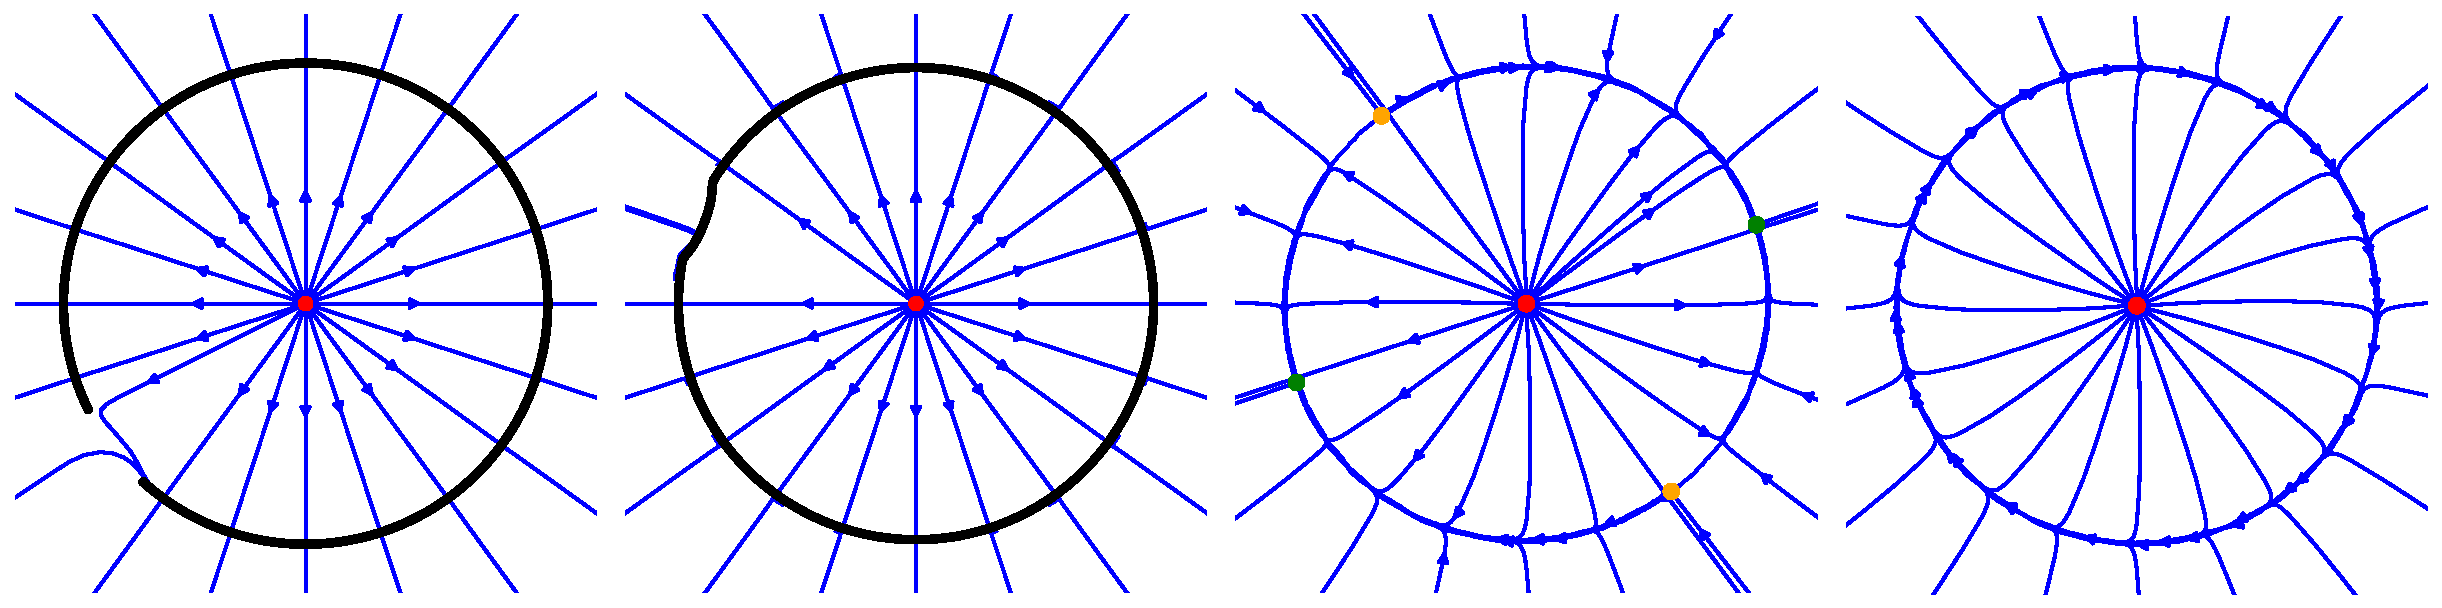
\includegraphics[width=.8\textwidth]{ring_perturbations_stream}
       \caption{Perturbations to a simple implementation of a ring attractor all leave the invariant manifold intact. % (Left)  Examples of a local perturbation to the vector field through the addition of a bump to the vector field along the ring attractor.
              (Leftmost) An example of a bump perturbation that results in the ring breaking up and becoming diffeomorphic to a line. %slow flow in hole?
              (Left, middle) An example of a bump perturbation that maintains the ring structure, but deforms it locally.
              %
      % (Right) Examples of a global perturbation to the vector field through the addition of a small term to the connectivity matrix. 
       (Right, middle) A global perturbation that results in a system with four fixed points along the persistent invariant manifold. %The two saddle nodes (yellow dots) are connected to the stable fixed points (green dots) through connecting orbits.
       (Rightmost)   A global perturbation that results in a limit cycle.}
         \label{fig:ring_activity_pert}
\end{figure}

%All perturbations maintain the invariant manifold.



\subsubsection{Finite-sized head direction network model}\label{sec:hd}
Continuous attractor models of the head direction representation suggest that the representation emerges from the interactions of recurrent connections among neurons that form a circular or ring-like structure \citep{zhang1996, Noorman2022, ajabi2023}. 
Since continuous attractors are susceptible to noise and perturbations the precise representation of the head direction can in principle easily be disrupted.
We will the implications of the Persistence theorem in the case of the implementation of a continuous ring attractor presented in \citep{Noorman2022}.
As this continuous ring attractor is bounded its invariant manifold persists and, hence, no divergent orbits are created under small perturbations to this system.
This model is composed of $N$ heading-tuned neurons  with preferred headings $\theta_j \in \{\frac{2\pi i}{N}\}_{i=1\dots N}$ radians.
For sufficiently strong local excitation (given by the parameter $J_E$) and broad inhibition, this network will generate a stable bump of activity, one corresponding to each head direction. This continuum of fixed points for a one dimensional manifold homeomorphic to the circle. 

\begin{figure}[H]
     \centering
  \includegraphics[width=\textwidth]{Noorman_perturbations}
       \caption{Perturbations to the ring attractor introduced in \citep{Noorman2022}. (Left)  Examples of a local perturbation to the vector field through the addition of a bump to the vector field along the ring attractor.
       (Leftmost) An example of a bump perturbation which cuts out a piece of the ring attractor, the stable fixed points of the system are shown in black. A heteroclinic orbit is created on the bounday of the hole with a slow flow.
       (Left, middle) An example of a bump perturbation that deforms the ring attractor, but maintains its topology.
       (Right) Examples of a global perturbation to the vector field through the addition of a small term to the connectivity matrix. }
         \label{fig:Noorman_ring_activity_pert}
\end{figure}


We evaluate the effect of perturbations on a network of size $N = 6$ with the optimal value $J_E^*=2.4$ through local and parametrized perturbations, similarly as for the toy ring attractor model.
The space of possible perturbations in Sec. ~\ref{sec:imt} is very large. To be able to form an image of what happens in the theorem we will work out the effect of some examples of perturbations. Hereby, we will focus on two kinds of perturbations, local and parametric. 
%Definition of a bump perturbation
We define a local perturbation (i.e., a change to the ODE with compact support) through the bump function $\Psi(x) = \exp\left(\frac{1}{\|x\|^2-1}\right)$ for $\|x\|<1$ and zero outisde, by multiplying it with a uniform, unidirectional vector field. 
%Definition of a global perturbationThe parametrized perturbations are characterized as the addition of random matrix to the connection matrix. 
We further investigate the effect of parameteric perturbations of the form if a term $\vW x$ to the original ODE with the entries of $\vW$ sampled from a normal distribution with mean zero and variance $\frac{1}{100}$. 
All such perturbations leave at least a part of the continuous attractor intact and preserve the invariant manifold, i.e. the parts where the fixed points disappear a slow flow appears.





\section{Discussion}
We have derived a general theory that describes the loss landscape of RNNs around continuous attractor solutions.
This theory implies backpropagating gradient does not explode for systems near compact continuous attractors because of divergent dynamics.
This insight also suggests that there can exist homeostatic mechanisms for certain implementations of continuous attractors that maintain the structure of the attractor sufficiently for the neural computation it is used in, which we demonstrate in simple networks.

%activation functions
It is well-known that activation functions play a critical role in propagating these gradients effectively through the network  \citep{jagtap2023, ramachandran2017, hayou2019}.
The activation function can have many forms.
The ones that are $C^r$ for $r\geq 1$ are the ones to which the Persistence Theorem applies. 
The Persistence Theorem further specifies how the smoothness of the activation can have implications on the smoothness of the persistence invariant manifold.
For situations where smoothness of the persistent invariant manifold is of importance, smoother activation functions might be preferrable, such as the Exponential Linear Unit (ELU)\citep{clevert2015} or the Continuously Differentiable Exponential Linear Units (CELU) \citep{barron2017}.




%\subsection{Footnotes}
%Footnotes should be used sparingly.  If you do require a footnote, indicate
%footnotes with a number\footnote{Sample of the first footnote.} in the
%text. Place the footnotes at the bottom of the page on which they appear.
%Precede the footnote with a horizontal rule of 2~inches (12~picas).
%
%
%Note that footnotes are properly typeset \emph{after} punctuation
%marks.\footnote{As in this example.}

%\begin{ack}
%Use unnumbered first level headings for the acknowledgments. All acknowledgments go at the end of the paper before the list of references. Moreover, you are required to declare
%funding (financial activities supporting the submitted work) and competing interests (related financial activities outside the submitted work).
%More information about this disclosure can be found at: \url{https://neurips.cc/Conferences/2023/PaperInformation/FundingDisclosure}.
%
%
%Do {\bf not} include this section in the anonymized submission, only in the final paper. You can use the \texttt{ack} environment provided in the style file to autmoatically hide this section in the anonymized submission.
%\end{ack}



%\section{Supplementary Material}
%
%Authors may wish to optionally include extra information (complete proofs, additional experiments and plots) in the appendix. All such materials should be part of the supplemental material (submitted separately) and should NOT be included in the main submission.


%\section*{References}
%The natbib package will be loaded for you by default. Citations may be author/year or numeric, as
%long as you maintain internal consistency. As to the format of the references themselves, any style is
%acceptable as long as it is used consistently

%References follow the acknowledgments in the camera-ready paper. Use unnumbered first-level heading for
%the references. Any choice of citation style is acceptable as long as you are
%consistent. It is permissible to reduce the font size to \verb+small+ (9 point)
%when listing the references.
%Note that the Reference section does not count towards the page limit.
%\medskip

\small

\newpage
\bibliographystyle{abbrvnat}
\bibliography{../cit,../catniplab}

\newpage
\section{Supplementary Material}

RNNs are also capable of learning complex patterns and relationships in the data, which makes them in particular useful as models for neural computations. This is achieved through the use of non-linear activation functions and the training of the network using backpropagation through time (BPTT).
BPTT allows the network to adjust the weights of the connections between neurons based on the error signal that is propagated backwards through time. 
%This makes them suitable models for 

However, training RNNs by using back-propagation through time to compute error-derivatives can be difficult.  Early attempts suffered from vanishing and exploding gradients \citep{kolen2001} and this meant that they had great difficulty learning long-term dependencies. 
Many different methods have been proposed for overcoming this difficulty.


\end{document}
